\documentclass[11pt,aspectratio=169]{beamer}
\usepackage[T1]{fontenc}
\usepackage[utf8]{inputenc}
\usepackage[english]{babel}
\usepackage{mathpazo}
\usefonttheme{serif}
\usepackage{amsmath,amssymb,booktabs,array,graphicx,microtype}
\usepackage{adjustbox}
\usepackage{tikz}
\usetikzlibrary{arrows.meta,calc,positioning,decorations.pathreplacing,patterns,fit,backgrounds}
\usepackage{animate}

% Figures and animations come from the idea folder; the TikZ figures in tikz/ are copies
% of those of the note.
\newcommand{\figdir}{../../ideas/group-identification/figures}
\graphicspath{{../../ideas/group-identification/figures/}}

% Colours of the note: i, j and a third flight; neutrals for text, grids and fills.
\definecolor{blueI}{HTML}{2A78D6}
\definecolor{orangeJ}{HTML}{EB6834}
\definecolor{aqua}{HTML}{1BAF7A}
\definecolor{ink}{HTML}{0B0B0B}
\definecolor{ink2}{HTML}{52514E}
\definecolor{muted}{HTML}{9A9893}
\definecolor{light}{HTML}{E6E5E1}
\definecolor{steel}{RGB}{74,96,121}
\definecolor{steellight}{RGB}{192,206,220}

\tikzset{
  >={Stealth[length=1.8mm]},
  every picture/.style={line cap=round, line join=round},
  track i/.style={blueI, line width=1.1pt},
  track j/.style={orangeJ, line width=1.1pt},
  track k/.style={aqua, line width=1.1pt},
  pt/.style={circle, inner sep=1.5pt, draw=ink, line width=0.4pt},
  pt i/.style={pt, fill=blueI},
  pt j/.style={pt, fill=orangeJ},
  pt k/.style={pt, fill=aqua},
  hollow j/.style={circle, inner sep=1.5pt, draw=orangeJ, fill=white, line width=0.9pt},
  lbl/.style={font=\footnotesize},
  note/.style={font=\footnotesize, text=ink2},
  tol/.style={draw=ink2, densely dashed, line width=0.5pt},
  flight/.style={circle, draw=ink, line width=0.6pt, minimum size=5.6mm, inner sep=0pt, font=\footnotesize, fill=white},
  inE1/.style={flight, fill=blueI, text=white},
  inE2/.style={flight, fill=orangeJ, text=white},
  edge/.style={ink, line width=1.2pt},
  bar/.style={draw=none, minimum height=3mm, inner sep=0pt},
  panel/.style={font=\small\bfseries, anchor=west},
}

\newcommand{\R}{\mathbb{R}}
\newcommand{\Z}{\mathbb{Z}}
\newcommand{\x}{\mathbf{x}}
\newcommand{\vh}{\hat{\mathbf{v}}}
\newcommand{\M}{\mathcal{M}}
\newcommand{\I}{\mathcal{I}}
\newcommand{\dep}{\mathrm{dep}}
\newcommand{\fin}{\mathrm{fin}}
\newcommand{\xc}{\mathrm{xc}}
\newcommand{\vis}{\mathrm{vis}}
\newcommand{\st}[1]{\textsf{#1}}
\newcommand{\ind}{\mathbf{1}}

% Theme: steel-blue title bar, white pages, as in the earlier decks.
\setbeamercolor{structure}{fg=steel}
\setbeamercolor{normal text}{fg=ink,bg=white}
\setbeamercolor{frametitle}{fg=white,bg=steel}
\setbeamercolor{alerted text}{fg=blueI}
\setbeamercolor{takeaway}{fg=steel,bg=steellight!30}
\setbeamercolor{defbox}{fg=ink,bg=steellight!28}
\setbeamersize{text margin left=7mm,text margin right=7mm}
\setbeamertemplate{navigation symbols}{}
\setbeamertemplate{itemize item}{\textcolor{steel}{\small$\bullet$}}
\setbeamertemplate{itemize subitem}{\textcolor{steel}{\textendash}}
\setbeamertemplate{itemize/enumerate body begin}{\setlength{\itemsep}{0.3em}}
\setbeamertemplate{frametitle}{%
  \nointerlineskip
  \begin{beamercolorbox}[wd=\paperwidth,ht=9mm,dp=3mm,center]{frametitle}
    \large\insertframetitle\strut
  \end{beamercolorbox}
  \begin{tikzpicture}[remember picture,overlay]
    \node[anchor=north east,text=white,inner sep=0pt,xshift=-2.3mm,yshift=-4.2mm]
      at(current page.north east){\small\insertframenumber};
  \end{tikzpicture}}
\setbeamertemplate{footline}{%
  \hspace{7mm}\textcolor{muted}{\fontsize{6.5}{8}\selectfont
    Matteo Di Sante\enspace|\enspace Group flight identification\enspace|\enspace xc-lab, 23 October 2026}\vspace{2mm}}

\newcommand{\source}[1]{\par\vspace{1mm}{\fontsize{7}{8.3}\selectfont\color{ink2}#1\par}}
\newcommand{\takeaway}[1]{\par\vfill
  \begin{beamercolorbox}[wd=\linewidth,sep=5pt]{takeaway}\small #1\end{beamercolorbox}}
% A definition: its name in bold, then the statement, on a pale band.
\newcommand{\defn}[2]{%
  \begin{beamercolorbox}[wd=\linewidth,sep=5pt]{defbox}\small\textcolor{steel}{\textbf{#1.}}\enspace #2\end{beamercolorbox}}
% A TikZ figure of the note, scaled to fit the given height and the line width.
\newcommand{\tikzfig}[2][0.8\textheight]{%
  \begin{center}\adjustbox{max width=\linewidth,max height=#1}{\input{tikz/#2}}\end{center}}
% An animation of the note; viewers without PDF JavaScript show its last frame.
\newcommand{\anim}[2]{\animategraphics[width=#1,controls={play,step,stop},loop,poster=last,
  timeline=\figdir/#2_frames.tln]{8}{\figdir/#2_frames}{}{}}
% A full-page divider that opens one part of the talk.
\newcommand{\partframe}[2]{%
\begin{frame}[plain,noframenumbering]
\begin{tikzpicture}[remember picture,overlay]
 \fill[steel](current page.south west)rectangle(current page.north east);
 \node[text=white,align=center,text width=.82\paperwidth]at([yshift=4mm]current page.center)
   {{\Large\bfseries #1}\\[3mm]{\normalsize\color{steellight}#2}};
\end{tikzpicture}
\end{frame}}

\hypersetup{pdftitle={Group flight identification},pdfauthor={Matteo Di Sante},
  colorlinks=true,urlcolor=blueI,linkcolor=blueI}

\begin{document}

\begin{frame}[plain]
\begin{tikzpicture}[remember picture,overlay]
 \fill[steel](current page.south west)rectangle(current page.north east);
 \fill[steellight](current page.south west)rectangle([yshift=20mm]current page.south east);
 \node[text=white,align=center,text width=.9\paperwidth]at([yshift=8mm]current page.center)
   {{\LARGE\bfseries Who flies with whom?}\\[4mm]
    {\large Identifying group flights in the FFVL archive}};
 \node[text=steel,align=center]at([yshift=10mm]current page.south)
   {{\normalsize Matteo Di Sante\quad|\quad xc-lab meeting, 23 October 2026}\\[1.5mm]
    {\footnotesize Method note and code: \texttt{xc-lab/ideas/group-identification}}};
\end{tikzpicture}
\end{frame}

\partframe{Part 1: the idea}{What the method does, on pictures}

\begin{frame}{The question}
\begin{beamercolorbox}[wd=\linewidth,sep=6pt,center]{takeaway}
\large For every flight and every instant: alone or in a group, and with whom?
\end{beamercolorbox}
\tikzfig[0.65\textheight]{requirements}
\end{frame}

\begin{frame}{The method in six steps}
\tikzfig[0.8\textheight]{overview_idea}
\end{frame}

\begin{frame}{Two pilots on one route, two minutes apart}
\begin{columns}[c,onlytextwidth]
\column{.66\textwidth}
\anim{\linewidth}{contact}
\column{.31\textwidth}
$j$ flies the route of $i$, 2~min later.
\par\bigskip
Same instant: \textbf{1~km apart}.
\par\bigskip
Same place, with a delay: \textbf{in contact}.
\end{columns}
\end{frame}

\begin{frame}{From contacts to groups: an example day}
\begin{columns}[c,onlytextwidth]
\column{.64\textwidth}
\anim{\linewidth}{example_day}
\column{.33\textwidth}
\small
\textbf{Group}: pilots linked by chains of contacts.
\par\medskip
\textbf{Configuration}: a group with the same members ($c_1,\dots,c_4$).
\par\medskip
\textbf{Episode}: configurations without a break (E1, E2).
\end{columns}
\end{frame}

\partframe{Part 2: the definitions}{The same steps, with formulas}

\begin{frame}{Start at the departure}
\tikzfig[0.55\textheight]{local}
\defn{Departure}{
\[
  k^\dep_i=\min\bigl\{k:\ \|\x_i(k)-\x_i(k^0_i)\|>R_\dep\bigr\},\qquad R_\dep=3~\text{km}.
\]
Before it: local phase \st{L}.}
\end{frame}

\begin{frame}{Correspondence: the same place at two instants}
\defn{Correspondence}{One clock (UTC) for all flights: $i$ at instant $t$, $j$ at instant
$t'=t+l$, with $l$ the delay:
\[
  (t,t')\in\M_{ij}\iff |t'-t|\le\delta,\ \ \|\x_i(t)-\x_j(t')\|<\varepsilon_h,\ \
  |z_i(t)-z_j(t')|<\varepsilon_z,\ \ D_{ij}(t,t')=1
\]}
\begin{columns}[c,onlytextwidth]
\column{.62\textwidth}
\tikzfig[0.5\textheight]{isotropic}
\column{.34\textwidth}
$\delta=2$~min\par
$\varepsilon_h=500$~m\par
$\varepsilon_z=300$~m
\par\bigskip
\small A group is flat: $\sim$1~km wide, a few hundred m high. A box keeps A and rejects B; one
3D radius rejects A or accepts B.
\end{columns}
\end{frame}

\begin{frame}{Headings count only when both pilots glide}
\tikzfig[0.45\textheight]{heading}
\defn{Heading condition}{
\[
  D_{ij}(t,t')=\begin{cases}
    \ind\bigl[\vh_i(t)\cdot\vh_j(t')>\cos\theta_{\max}\bigr] & \text{if both pilots glide},\\
    1 & \text{otherwise,}
  \end{cases}\qquad \theta_{\max}=45^\circ.
\]}
\end{frame}

\begin{frame}{Contact: the two shadows of $\M_{ij}$}
\defn{Contact}{
\[
  m_{ij}(t)=\ind\bigl[\exists\,t':(t,t')\in\M_{ij}\bigr],\qquad
  m_{ji}(t')=\ind\bigl[\exists\,t:(t,t')\in\M_{ij}\bigr],\qquad
  a_{ij}=m_{ij}\vee m_{ji}
\]}
\begin{center}
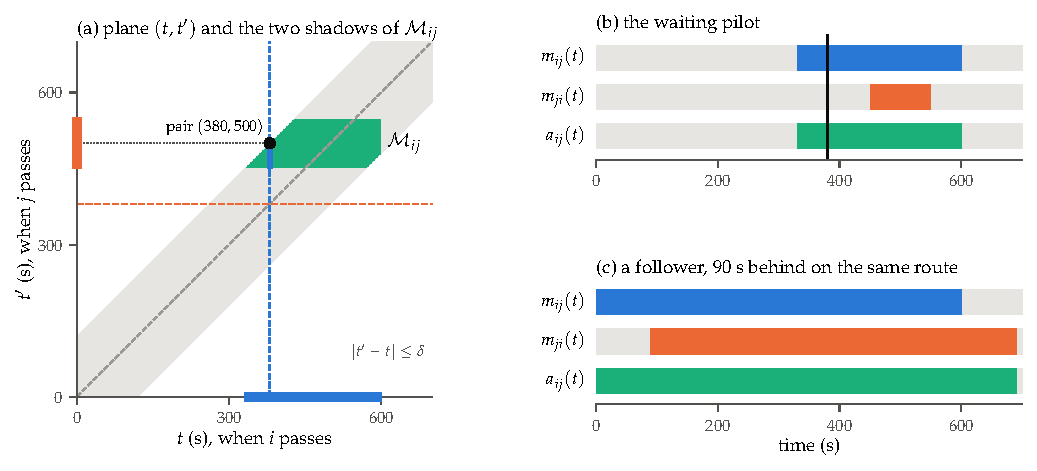
\includegraphics[width=\linewidth,height=0.5\textheight,keepaspectratio]{asymmetry_plane.pdf}
\end{center}
\source{(b) $i$ waits in a thermal that $j$ crosses. (c) $j$ follows $i$ 90~s behind.}
\end{frame}

\begin{frame}{Pair intervals: fill short gaps, drop short contacts}
\tikzfig[0.5\textheight]{pair_intervals}
\defn{Pair interval}{A run of $a_{ij}=1$ with gaps $<g=120$~s joined, kept if it lasts
$\ge\tau^*=38.1$~min: $[t_{\rm on},t_{\rm off})$.}
\source{$\tau^*$: at most one interval in ten is chance, on pairs shifted in time (second deck,
\emph{Is it chance?}).}
\end{frame}

\begin{frame}{Contact is not transitive: cut the graph instant by instant}
\tikzfig[0.45\textheight]{transitivity}
\defn{Active graph}{
\[
  G(t)=\bigl(V(t),E(t)\bigr),\qquad
  E(t)=\bigl\{\{i,j\}:\ t\in[t_{\rm on},t_{\rm off})\bigr\},\qquad
  V(t)=\text{flights in the air}.
\]
A \textbf{group} at $t$: a connected component of $G(t)$ with two or more flights.}
\end{frame}

\begin{frame}{Configuration: a group with fixed members}
\tikzfig[0.4\textheight]{configurations}
\begin{columns}[T,onlytextwidth]
\column{.49\textwidth}
\defn{Configuration}{$c=\bigl(M_c,[t^{\rm start}_c,t^{\rm end}_c)\bigr)$: $M_c$ is a group of
$G(t)$ at every $t$ of the interval, and the interval is maximal.}
\column{.49\textwidth}
\defn{Membership}{
\[
  \gamma_i(t)=\begin{cases}
    \st{L} & \text{before the departure},\\
    c & i\in M_c,\ t\in[t^{\rm start}_c,t^{\rm end}_c),\\
    \st{S} & \text{otherwise (solo).}
  \end{cases}
\]}
\end{columns}
\end{frame}

\begin{frame}{Episode: a chain of configurations}
\tikzfig[0.5\textheight]{episodes}
\defn{Episode}{A connected component of the links
\[
  c\to c'\iff t^{\rm start}_{c'}=t^{\rm end}_c\ \wedge\ M_c\cap M_{c'}\ne\emptyset .
\]}
\end{frame}

\begin{frame}{Dependency block: the flights tied by episodes}
\tikzfig[0.5\textheight]{blocks}
\defn{Block}{A connected component of the graph flights--episodes of a day. The bootstrap
resamples whole blocks.}
\end{frame}

\begin{frame}{Who follows whom: a label, not used to build the groups}
\begin{columns}[c,onlytextwidth]
\column{.62\textwidth}
\anim{\linewidth}{altitude_clock}
\column{.35\textwidth}
\small
The contact needs only that some delay exists; to say who is ahead we need its value. At $t$,
the delay at which $j$ passes closest to where $i$ is (Li et al.):
\[
  l^*(t)=\arg\min_{l}\,\|\x_i(t)-\x_j(t+l)\|
\]
$\ell_{\rm med}=\mathrm{median}\,l^*$ over a pair interval; $\ell_{\rm med}>0$: $j$ follows $i$.
\par\medskip
\textbf{Glide}: one sharp minimum.\par
\textbf{Thermal}: one per turn; altitude leaves $\Delta z/w\pm150$~s, against $\delta=120$~s.\par
\textbf{Search}: left out.
\end{columns}
\end{frame}

\begin{frame}{On the FFVL archive}
\begin{columns}[t,onlytextwidth]
\column{.24\textwidth}
\centering
{\Huge\textcolor{blueI}{21.7\%}}\par\smallskip
\small of paraglider flights fly in a group at some point
\column{.24\textwidth}
\centering
{\Huge\textcolor{orangeJ}{6.9\%}}\par\smallskip
\small of hang-glider flights
\column{.24\textwidth}
\centering
{\Huge\textcolor{steel}{17\,169}}\par\smallskip
\small episodes
\column{.24\textwidth}
\centering
{\Huge\textcolor{steel}{58 min}}\par\smallskip
\small median episode; 2 flights (median), up to 53
\end{columns}
\source{160\,637 flights; $\delta=2$~min, $\varepsilon_h=500$~m, $\varepsilon_z=300$~m, $g=120$~s,
$\tau^*=38.1$~min.}
\end{frame}

\begin{frame}{Episodes: how long, how many flights}
\begin{center}
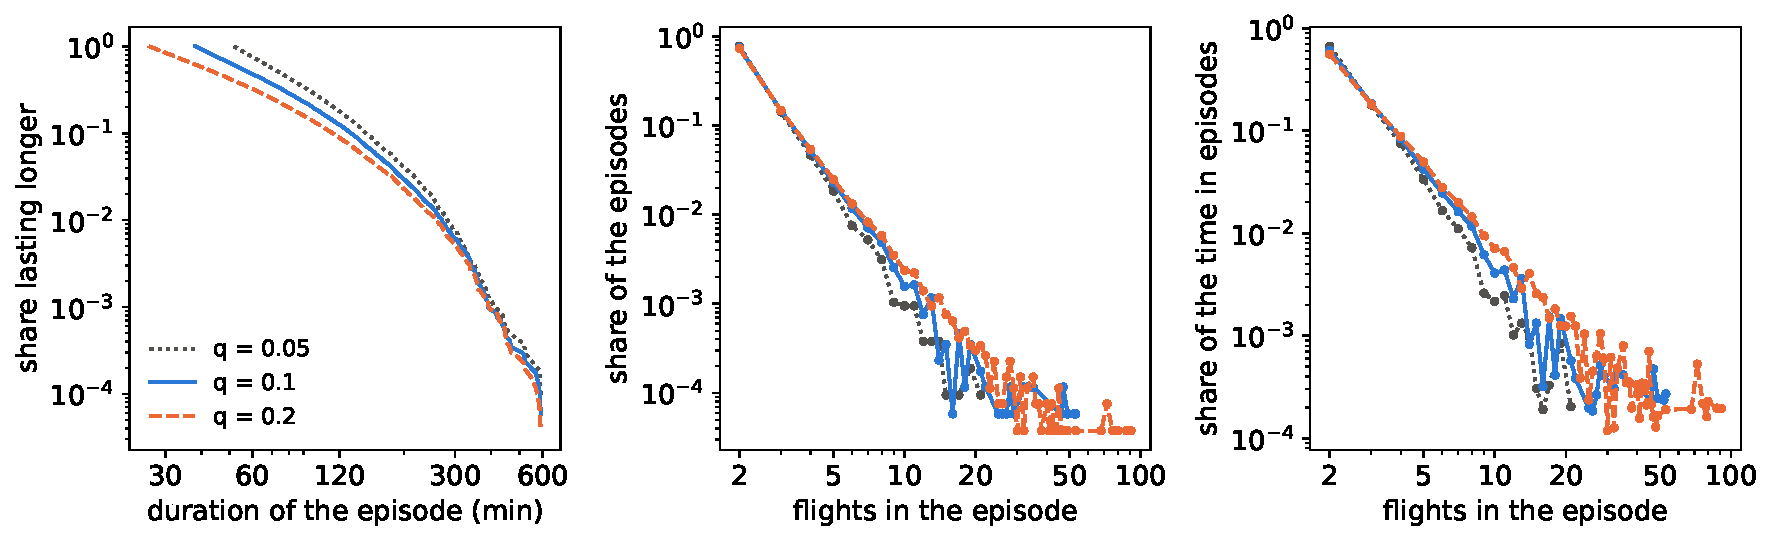
\includegraphics[width=\linewidth,height=0.5\textheight,keepaspectratio]{assessment_structure_episodes.pdf}
\end{center}
\source{Whole archive, $\delta=2$~min. Left: share lasting longer. Middle: share of the episodes
of each size. Right: share of the episode time. Size: distinct flights of the episode.}
\takeaway{With $q=0.1$ the median episode lasts 58~min and 74\% are pairs. Weighted by time
the pairs drop to 61\%: large episodes last longer.}
\end{frame}

\begin{frame}{Configurations: how long, how many pilots at once}
\begin{center}
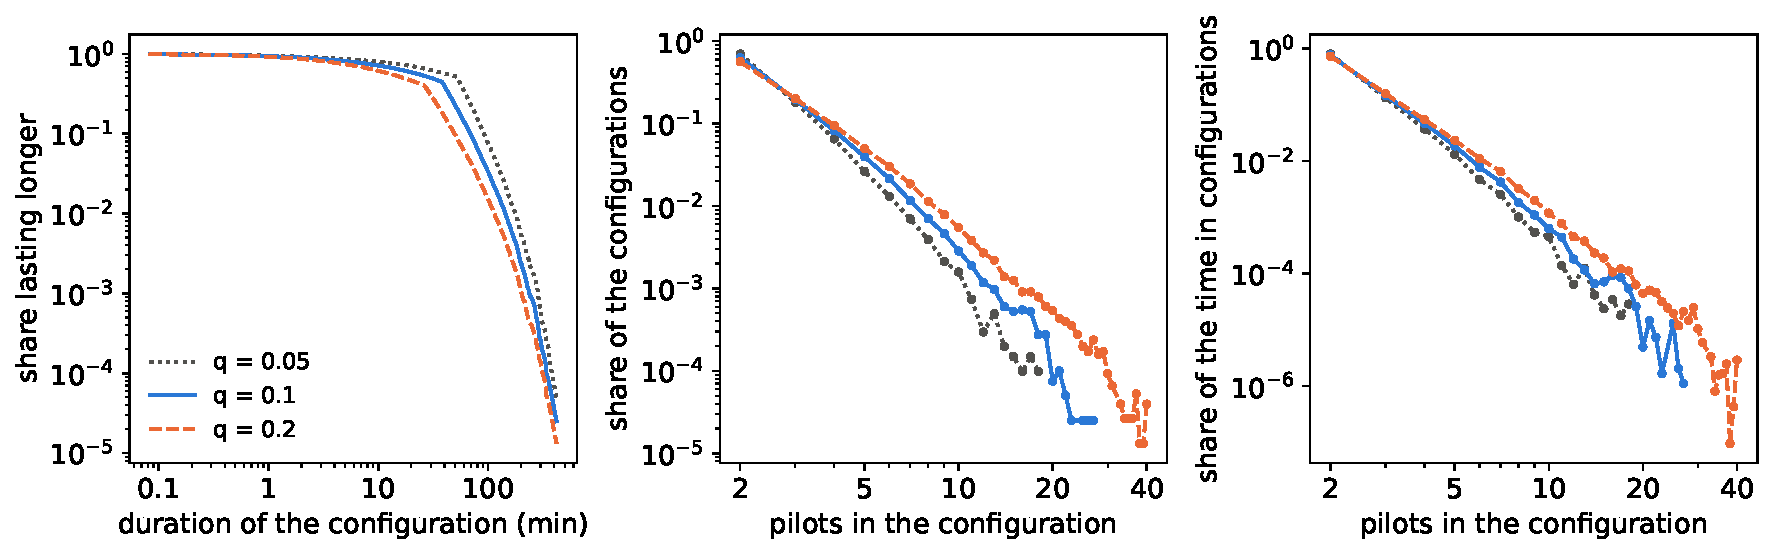
\includegraphics[width=\linewidth,height=0.5\textheight,keepaspectratio]{assessment_structure_configurations.pdf}
\end{center}
\source{Whole archive, $\delta=2$~min. A configuration keeps its members; each arrival or
departure starts a new one. Size: pilots at once.}
\takeaway{Median configuration 30~min, 63\% are pairs. Weighted by time the pairs rise to
77\%: large configurations change quickly.}
\end{frame}

\end{document}
